\chapter{Testy}\label{cha:pierwszyDokument}

Ogolnie :
zlozonosc algorytmu, zajmowana pamiec

Poszczegolnych:
szybkosc funkcji, odchylenie standardowe , srednie itp z np 20 runów, runy zrobic tez dla roznych ilosci iteracji bo moze sie cos nie wyrabia i potem jest lepiej 
%---------------------------------------------------------------------------

\section{Metody selekcji}\label{sec:strukturaDokumentu}

Analiza metod selekcji w obrębie jednej instancji została przeprowadzona przy założeniu stałych takich jak:
\begin{itemize}
\item
 warunki początkowe, a więc stałej macierzy odległości, macierzy przepływu oraz początkowej populacji,
\item
metoda selekcji,
\item
metoda krzyżowania,
\item
ilość iteracji algorytmu
\end{itemize}
\par
\vspace{0,4cm}
Testy zostały przeprowadzone dla poniższych instancji danych wejściowych. W celu uzyskania ostatecznego rozwiązania, a więc rozwiązania nie zmieniającego się już pod wpływem kolejnych iteracji algorytmu, analiza została przeprowadzona dla odpowiednio 20 000 oraz 50 000 iteracji.\\

\subsection{Dane wejściowe instancja I}




\begin{itemize}
\item 20 000 iteracji\\
\par
 W \ref{instancja_1} zostały zestawione wartości funkcji celu w kolejnych iteracjach dla poszczególnych metod selekcji. Metody selekcji zostały szczegółowo opisane w \ref{metody_selekcji}. Następnie dla każdej z metod została policzona średnia wartość funkcji celu, odchylenie standardowe oraz współczynnik zmienności będący stosunkiem wartości odchelenia standardowego i średniej. Za pomocą tych narzędzi statystycznych można określić zachowanie poszczególnych metod oraz wyodrębnić metodę dającą w tym kontekście najbardziej satysfakcjonujący wynik. Kolorem zielonym zostałČ również zaznaczony najlepszy otrzymany wynik.\\
\par
\begin{table}[h!]
\begin{center}
\scalebox{0.6}{
\begin{tabular}{|c|c|c|c|c|c|c|c|c|}
\hline
\textbf{Iteracja}  &\textbf{Losowa}  & \textbf{Rankingowa} & \textbf{Ruletka} & \textbf{Turniejowa} & \textbf{Elitarna} & \textbf{Random 2} & \textbf{Rankingowa 2} & \textbf{Turniejowa 2}\\
\hline
 \textbf{1}&1676	&1662&1700&1666&1686&1688&1668	&1760 \\
\hline
 \textbf{2}&1680	&1662&1664&1666&1676&1682&1682&1756 \\
\hline
 \textbf{3}&1668	&1664&1710&1672&1680&1682&1672&1796  \\
\hline
 \textbf{4}&1666	&1664&1694&1696&1682&1680&1702	&1742  \\
\hline
 \textbf{5}&1666&1672&1692&1706&1692&1672&	1672&1820  \\
\hline
 \textbf{6}&1670	&1660&1706&1680&1670&1682&1670&1798\\
\hline
 \textbf{7}&1666&1666&1708&1690&1670&1680&1702&1766 \\
\hline
 \textbf{8}&1670	&1656&1722&1676&1668&1688&1686	&1700\\
\hline
 \textbf{9}&1692	&1666&1662&1656&1680&1708&1678	&1706\\
\hline
 \textbf{10}&1668	&1656&1670&1676&1674&1716&1706	&1826\\
\hline
 \textbf{11}&1682	&1660&1688&1670&1690&1712&1682	&1778 \\
\hline
 \textbf{12}&1696	&1660&1716&1688&1678&1728&1660	&1770 \\
\hline
 \textbf{13}&1668	&\color{green}\textbf{1654}&1692&1688&1684&1702&1672	&1774 \\
\hline
 \textbf{14}&1668	&1660&1668&1672&1706&	1696	&1698&1728\\
\hline
 \textbf{15}&1696	&1664&1672&1688&1684&	1684	&1684&1806\\
\hline
 \textbf{16}&1714	&1660&1686&1676&1674&	1676	&1690&1774\\
\hline
 \textbf{17}&1662&1656&1700&1674&1676&	1684	&1684&1758 \\
\hline
 \textbf{18}&1678	&1662&1672&1672&1690&	1692	&1680&1746\\
\hline
 \textbf{19}&1670	&1666&1718&1680&1680&	1712	&1662&1762\\
\hline
 \textbf{20}&1684&1660&1682&1666&1674&	1666	&1670&1720\\
\hline
 \textbf{ŚREDNIA}&1677	&1661&1691&1677&1680&	1691	&1681&1746\\
\hline
 \textbf{ODCHYLENIE STANDARDOWE}&13,15	&4,19&18,35&11,56&8,86&	16	&13,02&33,9\\
\hline
 \textbf{WSPÓŁCZYNNIK ZMIENNOŚCI}&0,78\%&0,25\%&1,09\%&0,69\%&0,53\%&0,95	\%&0,77\%&1,92\%\\
\hline
\end{tabular}}
\caption{Wartości funkcji celu dla poszczególnych metod selekcji}
\label{instancja_1}
\end{center}
\end{table}


\begin{figure}[h]
		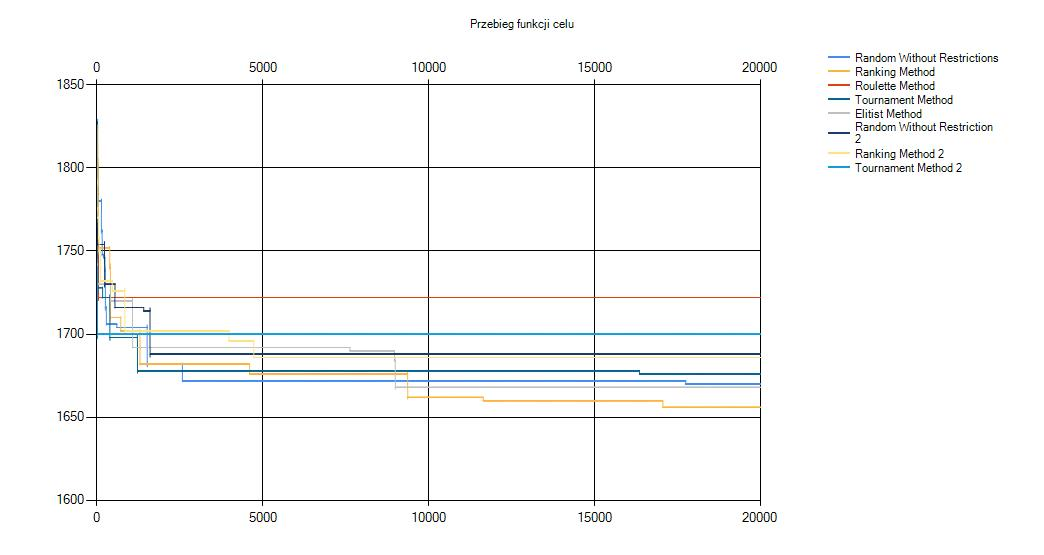
\includegraphics[scale=0.5]{../../../../Screeny/wszystkie_1656.jpg}
		\caption{Rozkład prawdopodobieństwa w metodzie rankingowej}
		\label{ranking}			
\end{figure}
\item 50 000 iteracji
\end{itemize}

\subsection{Dane wejściowe instancja II}